\section{Zielsetzung}
Dieser Versuch befasst sich mit der Leerlaufspannung sowie dem Innenwiderstand verschiedener Spannungsquellen.
\section{Theorie}
Unter einer Leerlaufspannung $U_0$ wird jene Spannung verstanden, die an einer Spannungsquelle anliegt, wenn kein Strom fließt. In einem Stromkreis, in dem ein Strom $I$ über einen Lastwiderstand $R_{\text{a}}$ fließt, ist 
jedoch eine sogenannte Klemmenspannung $U_{\text{k}}$ messbar, welche kleiner als $U_0$ ist. Grund hierfür ist der Innenwiderstand $R_{\text{i}}$ der Spannungsquelle. Genauer kann dies mithilfe des zweiten Kirchoffschen Gesetzes,
der Maschenregel, erklärt werden. Diese besagt, dass die Summe aller Spannungen in einer Masche gleich der Leerlaufspannung ist. Mit
   \begin{equation*}
   U = R\cdot I
   \end{equation*}
folgen hieraus die Gleichungen für Leerlaufspannung $U_0$ und Klemmenspannung $U_{\text{k}}$ für den in diesem Versuch gegebenen Schaltkreis (Vgl. Abbildung \eqref{fig:ersatzschaltbild}):
   \begin{equation*}
   \begin{aligned}
   U_0 &= IR_{\text{i}} + IR_{\text{a}}, \\
   U_{\text{k}} &= IR_{\text{a}} = U_0 - IR_{\text{i}}.
   \end{aligned}
   \end{equation*}
Es fällt auf, dass für die Messung der Leerlaufspannung ein hochohmiges Voltmeter nötig ist, damit $IR_{\text{i}}$ wegen des schwachen Stroms vernachlässigbar klein wird. Damit folgt dann $U_0 \approx U_{\text{k}}$.
 \begin{figure}[h!]
   \centering
   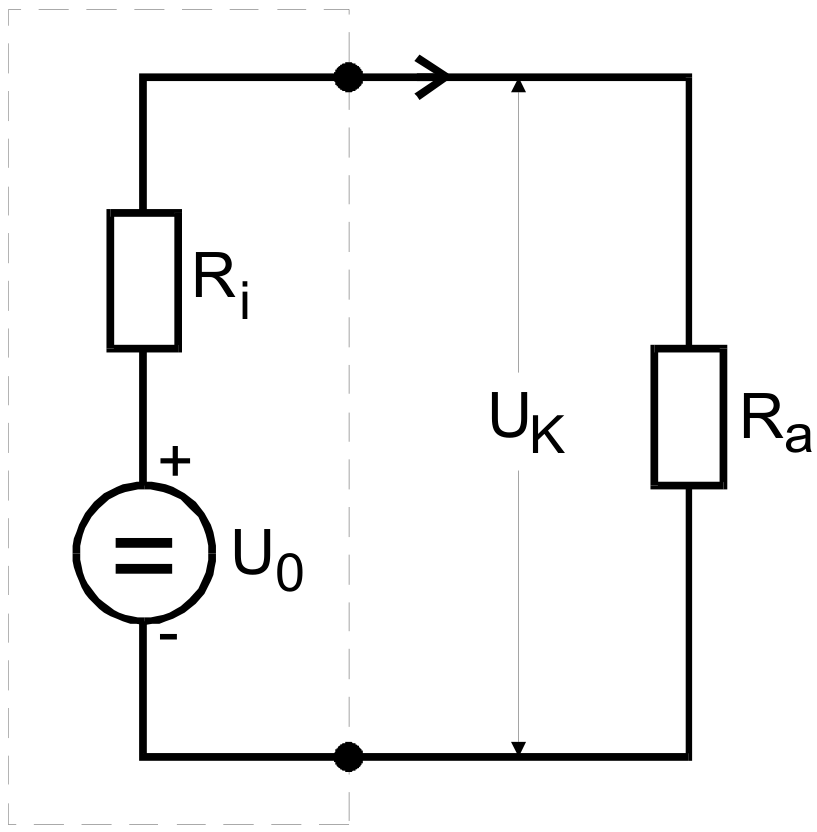
\includegraphics[width=0.4\linewidth]{ersatzschaltbild.png}
   \caption{Ersatzschaltbild einer realen Spannungsquelle mit Lastwiderstand.}
   \label{fig:ersatzschaltbild}
   \end{figure}

Um eine reale Spannungsquelle beschreiben zu können wird diese in einem Ersatzschaltbild durch eine ideale Spannungsquelle, die keinen Innenwiderstand besitzt, sowie einen ohmschen Widerstand $R_{\text{i}}$ dargestellt, welche
in Reihe geschaltet sind. Der Widerstand bewirkt, dass es eine begrenzt entnehmbare Leistung gibt, die durch
   \begin{equation*}
   N = I^2 R_{\text{a}} = N(R_{\text{a}})
   \end{equation*}
gegeben ist. Dabei wird die Leistung $N$ maximal, wenn $R_{\text{a}} = R_{\text{i}}$. Dieser Fall wird Leistungsanpassung genannt.
Bei elektrischen Generatoren ist der Innenwiderstand nicht zwingendermaßen durch einen parallelliegenden Gleichstromwiderstand gegeben, sondern durch einen Rückkopplungsmechanismus.
Dabei beeinflussen Änderungen des Belastungsstroms die Spannungsquelle. Somit muss der Innenwiderstand als differentielle Größe dargestellt werden:
   \begin{equation*}
   R_{\text{i}} = \frac{\symup{d} U_{\text{k}}}{\symup{d}I}.
  \end{equation*}
